\section{PS2b: Sokoban Game Mechanics}\label{sec:ps2b}
\graphicspath{{ps2b}}
\subsection{Discussion:}\label{sec:ps2b:disc}
This assignment was implementing the actions, mechanics, and dynamism into the game. By transferring the player, the boxes, and the locations into vectors or pairs, it made it very easy to search and validate locations. It also made it very easy to move pieces to new location. The search and move features were very important and helpful for establishing the edge cases in the game. 

\subsection{Key algorithms, Data structures and OO Designs used in this Assignment:}\label{sec:ps2b:kdo}
  In this assignment as mentioned prior, I put the pieces and the locations into vectors. I coupled this choice with an easily integrated function from the standard library find if, this takes iterators as well as functors. The functor I applied would check certain locations and return the iterator or the end depending on the input. This was very helpful for the not only checking the wall locations, but also checking if there were multiple boxes in front of each other. 
  
 Here is an excerpt from the code, I implemented a while loop with the find if function to simulate moving the line of boxes. 

              \textbf{\colorbox{lime}{ code:}}
       \begin{lstlisting}
       while(x != boxLocation.end())
                {
                    if(map[playerLocation.first - (i+1)][playerLocation.second] == '.' || map[playerLocation.first - (i+1)][playerLocation.second] == 'a')
                    {
                        boxes.push_back(*x);
                    }
                    i++;
                    x = find_if(boxLocation.begin(), boxLocation.end(), [this,i](pair<int,int> p){return p.first == playerLocation.first - i && p.second == playerLocation.second;});
                }
                if(map[playerLocation.first - (i)][playerLocation.second] == '.' || map[playerLocation.first - (i)][playerLocation.second] == 'a')
                {
                    for(auto y : boxes)
                    {
                        vector<pair<int,int>>::iterator x = find_if(boxLocation.begin(), boxLocation.end(), [y](pair<int,int> p){return p.first == y.first && p.second == y.second;});                        
                        x->first--;
                    }
                    playerLocation.first--;
                }

       \end{lstlisting}
\subsection{What I learned :}\label{sec:ps2b:learn}
I learned how to implement features that have higher levels of complexity. Adding the feature of multiple boxes took a certain level of implementation. I also learned how to use lambda functions and to take advantage of the already implemented algorithms in the standard library. I also learned how to lint my code, and what proper programming looks like. 

\newpage
\subsection{Codebase}\label{sec:ps2b:code}

\colorbox{pink}{\textbf{Makefile:}} \newline \textbf{This Makefile contains the linting too.}
\lstinputlisting[language=Make]{ps2b/Makefile}


\colorbox{pink}{\textbf{main.cpp}} \lstinputlisting{ps2b/main.cpp}

\colorbox{pink}{\textbf{Sokoban.h}} 
\lstinputlisting{ps2b/Sokoban.h}

\colorbox{pink}{\textbf{Sokoban.cpp}} 
\lstinputlisting{ps2b/Sokoban.cpp}



\subsection{Output:}\label{sec:ps2b:output}
\begin{figure}[h]
    \centering
    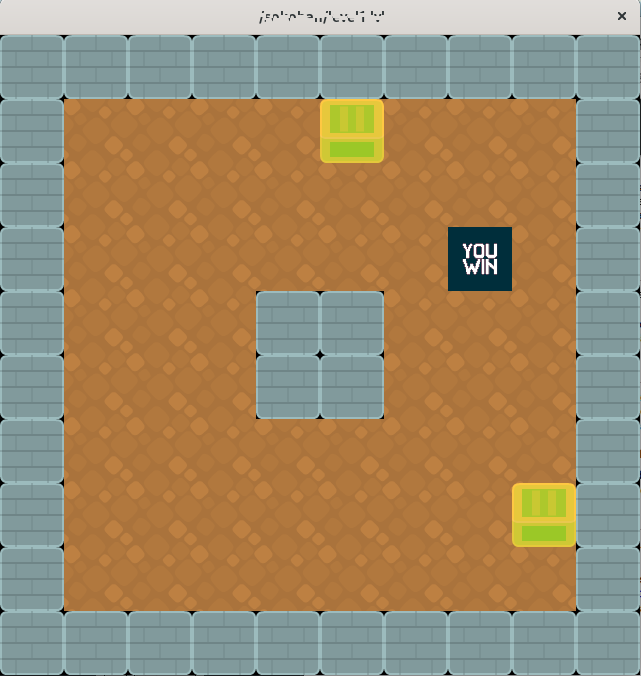
\includegraphics[width=0.7\textwidth]{projectPictures/PS2b.png}
    \caption{Player wins game}
    \label{fig:ps2b}
\end{figure}

